As this thesis aims to offer an open-source framework for VR surgery, the most obvious choice for hardware was used.
A combination of commercially available HMDs and open-source software is used to develop an easily accessible framework.
For this thesis, the HTC Vive \cite{Vive} together with the recent Valve Index Controller \cite{ValveIndex} were used.
However, any commercially available headset and controller which is compatible with SteamVR will work with this system.
OpenVR \cite{OpenVR} (also calles SteamVR), the from Steam developed open-source framework for VR development, abstracts the HMD and specifics of controllers for the end user.
By utilizing SteamVR, requirement \ref{req::N9} is practically ensured.

Since running virtual reality software is computationally expensive, a desktop computer with the following hardware is recommended to comply with the given robustness and responsiveness requirements (\ref{req::N4}, \ref{req::N6}):

\begin{compactenum}[label=(\alph*)]
    \item Graphics Card: Nvidia GTX 1060 or equivalent
    \item CPU: Intel i5-4590 / AMD Ryzen5 1500X
    \item Memory (RAM): 8GB+
\end{compactenum}

%SteamVR
The VR software was developed using Unity3D (LTS 2018.4), which is broadly accepted by the community and seen as an easy to learn tool, with many tutorials and community support for learning \cite{bartneck2015robot}.
\\ Inside of Unity, the OpenVR Toolkit provided by SteamVR is used.
SteamVR consists of an interaction system in which button presses are mapped to actions.
By implementing features with actions instead of button presses in mind, controls are abstracted for any kind of input device.
Mappings can then be customized to user needs, although defaults are available for every controller supported.
\\ Additionally, the interaction system found in SteamVR will be utilized for this thesis, as it provides many functionalities to comply with requirement \ref{req::N2}.
Mentioned requirements (\ref{req::F2}) for locomotion could also be implemented through SteamVR.
Users can navigate by simply walking inside of the tracking space.
Full "walkability" can be realized by utilizing a OT sized tracking space.
To complement natural walking in smaller spaces, teleportation is realized by pressing the teleportation button to visualize a teleport area and teleport destination.
When letting go of the button, the user will teleport to the destination.
Obstructed or non available destinations are visualized through a red cross at the teleport destination.
Turning of the users field of vision is realized via "Snap Turn", in which the users view rotates by 45 degrees to the left or right.
Snap turn, in contrast to continuously rotating alternatives such as "Smooth Turn", has shown to work best to avoid nausea, especially for VR first timers. 
\\ Additionally, SteamVRs interaction toolkit allows for natural hand interaction.
By using SteamVR, virtual hands are projected into the VR.
Important to note is that Steam, the platform on which SteamVR is running, has to be running in the background for this to work.
Otherwise, the virtual hands will not appear inside of Unity3D.
\\ According to button input, the poses of the virtual hands change so that users can understand the underlying intentions of button presses.
For example, by pressing the grip button on the HTC Vive Controller, the virtual hand will make a grab motion with middle, ring and pinky finger.
In the case of the Valve Index Controller, real-time finger tracking allows for a full representation of the users hands in VR.
Any movement of the fingers is translated to the virtual hand.
A grab action is performed by grabbing the controller with middle, ring and pinky finger, in contrast to pressing a grip button.
\\ It follows, that a natural interaction system where moving your hands to interact with the environment has been implemented (Requirements \ref{req::N2}, \ref{req::F3}).
Users are able to interact with surgical instruments, the patient and the environment via their virtual hands.
Objects are selected by hovering over them and then grabbed by performing a grab motion with the Valve Index Controller or pressing the respective button on other input devices.
This way, objects can be easily rotated and moved inside of the OT.
A bare minimum of buttons is used to perform the procedures.
Solely the Graphical User Interface (GUI) and the execution of procedures is performed by pressing their respective button.

\begin{figure}[ht]
    \centering
    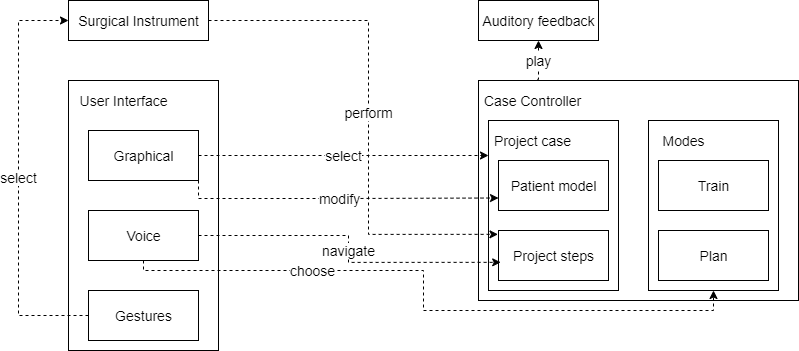
\includegraphics[width=375px]{images/implementation/architecture.png}
    \caption{\label{fig::ImplementationArchitecture}High-level overview of the applications architecture. Interactions between system components are visualized.}
\end{figure}

The broad overview of how individual system components interact with each other is depicted in Figure \ref{fig::ImplementationArchitecture}.
The CaseController component is responsible for handling all project case related information.
Via the GUI, users load a project case into the CaseController.
Inside of the CaseController, users can choose to switch the currently active mode via the VUI.
The mode will decide how steps, which are added by the user via the currently selected surgical instrument, are handled inside of the CaseController.
In planning mode, steps are directly added to the project case, while in training mode the correct execution of the procedure will be checked.
Either way, the CaseController calls the Auditory Feedback component to play auditory confirmations or errors to the user.
Surgical instruments are abstracted in such a way, that it does not matter which is currently selected for the CaseController.
New steps get passed to the CaseController in form of their 3D model with a new material attached to it.
